\chapter{Hyperparameter Tuning}
\label{chap:hyperparameter_tuning}
In this chapter, we will incrementally move to an optimized Genetic Algorithm

\section{No Free Lunch Theorem}
No Free Lunch Theorem:
The best hyperparameter settings of a Genetic Algorithm are very problem specific. \cite{kacprzyk_parameter_2007}, \cite{dao_maximising_2016} \todo{More ref}

\section{Start Scenario}

\section{Population}
\label{chap:hyperparameter_tuning:population}
The number of Individuals is of high importance to a genetic algorithm, as has been explained in section \ref{chap:foundation:genetic_algorithm}. Especially considering the limed processing resources available, a suitable population size has to be found. On one hand, a population that is too low might result in less diverse runs of the genetic algorithm, on the other hand, if population is too high, the simulations will become too costly. Considering these points, the first step of the hyper parameter tuning was to find a suitable population size. In the next chapter \ref{chap:hyperparameter_tuning:other_parameter}, we will aim to improve the hyperparamter using a more robust approach.

In order to test for the best population size, the other hyperparameters have to be assumed using an educated guess. While reviewing the literature, trends of general settings for genetic algorithms can be found. However \cite{mills_determining_2015} highlight the inconsistencies between findings, stating to have "uncovered conflicting opinions and evidence regarding key GA control parameters". 

However \cite{grefenstette_optimization_1986} suggests, that "while it is possible to optimize GA control parameters, very good performance can be obtained with a range of GA control parameter settings." 
This is also complimented by findings from \cite{kacprzyk_parameter_2007}: "The key insight from such studies is the robustness of EAs with respect to their parameter settings. Getting “in the ball park” is generally sufficient for good EA performance. Stated another way, the EA parameter “sweet spot” is reasonably large and easy to find [18]. As a consequence most EAs today come with a default set of static parameter values that have been found to be quite robust in practice."

Chosing the right selection method is complicated as well, as discuees by \cite{kacprzyk_parameter_2007}:
"One source of difficulty here is that selection pressure is not as easy to “parameterize” as population size. We have a number of families of selection procedures (e.g, tournament selection, truncation selection, fitness-proportional selection, etc.) to choose from and a considerable body of literature analyzing their differences (see, for example, [19] or [15]), but deciding which family to choose or even which member of a parameterized family is still quite difficult, particularly because of the interacting effects with population size [13]."

Looking at the literature might lead to hyperparameters are used that at least sufficient enough, to get an idea which range for population size is suitable. We will now look at different concrete hyperparameter suggestions from the literature.

\subsection{Suggested hyperparameter from the literature}
\todo{Use best values also from : Using genetic algorithms for automating automated lane-keeping system testing}
\todo{Talk about rules (e.g. 1/n for mut rate...) - look at: Parameter selection in genetic algorithms}
In an often cited thesis by \cite{de_jong_analysis_1975}, the following parameters have been suggested:
GA(50, 0.6, 0.001, 1.0, 7, E) These suggested parameters have been used successfully by various different genetic algorithms \cite{grefenstette_optimization_1986}. 

An extensive study by \cite{mills_determining_2015} which that took over "over 60 numerical optimization problems." into consideration found that "the most effective level settings found for each factor: population size = 200, selection method = SUS, elite selection percentage = 8\%, reboot proportion = 0.4, number of crossover points = 3, mutation rate = adaptive and precision scaling = 1/2 as fine as specified by the user."

\cite{grefenstette_optimization_1986} claim that GA(30, 0.95, 0.01, 1.0, 1, E) and GA(80, 0.45, 0.01, 0.9, 1, P) produced the best results. They also advised against, a mutation rate of over 0.05, suggesting poor performance. Using a low mutation rate is also suggested by \cite{whitley_genetic_1994} and \cite{jinghui_zhong_comparison_2005}. 
On the other hand, \cite{boyabatli_parameter_2004} state, that "Controversial to existing literature on GA, our computational results reveal that in the case of a dominant set of decision variable the crossover operator does not have a significant impact on the performance measures, whereas high mutation rates are more suitable for GA applications."
Other paper also find a relatively high mutation rate useful. \cite{almanee_scenorita_2021} uses genetic algorithms in a similar domain as this thesis. There, a Population of 50, crossover of 0.8 and mut of 0.2 was used. These used params are the same as the default params from deap (pop = 50 CXPB, MUTPB, NGEN = 0.5, 0.2, 4). \todo{cite https://deap.readthedocs.io/en/master/overview.html}

\cite{srinivas_genetic_1994} state, that for a higher population, cross : 0.6, mut: 0.001 and pop: 100 is a good starting point, while a lower population needs higher crossover and mutation rates like this cross: 0.9, mut: 0.01, pop: 30

These next three paper use ANOVA analysis to come a conclusion. \cite{fazal_estimating_2005} recommend:
Migration direction: Forward
Population size: 50 
Fitness scaling function: Rank
Selection function: Tournament
Elite count: 5
Crossover fraction: 0.5
Crossover function: Scattered


\cite{dao_maximising_2016} suggests these values after anova:
Migdirection: forwards
pop size: 200
fitness scaling: rank
selection: roulette
elite count: 1
Crossover prop: 0.7
MutationFunc: Gaussian
Crossover FUnc: two point
hybrid function: none


\cite{assistant_professor_amity_university_jaipur_rajasthan_india_parameter_2019} use these values after anova:
Direction: Forward
Pop: 200 
Fitness Scaling Function: linar Shift
selection: Roulette 
elite count: 10 
Crossover: 0.4 
Mutation: Constraint Dependent 
Crossover function: Heuristi
Hybrid Function: None




\subsection{results}
This now leads to a difficult decision in choosing the right parameters. Based on the extensive research, we will compare population size of 32, 48, 64 and 96. We will compare the different crossover rates: 0.8 and 0.6. For mutation, 0.01 and 0.2 will be discussed. Further we will use tournament selection with 2 and 4.
Each run will be executed 5 times to get rid of randomness and to make the results more robuts. We will run each simulation for 40 Generations.

\begin{figure}[!h]
	\centering
\begin{tabular}{ |l||c|c|c|c|  }
	\hline
	\multicolumn{5}{|c|}{ Comparison of Population Size} \\
	\hline
	Settings & 32 & 48 & 64 & 96\\
	\hline
	C: 0.6, M: 0.01, TS: 2   	& 3056(2955) & 1000(1000) & 1000(1000) & 1000(1000)\\
	C: 0.6, M: 0.01, TS: 4		& 3112(2981) & 1000(1000) & 1000(1000) & 1000(1000)\\
	C: 0.6, M: 0.2, TS: 2 		& 3129(2839) & 1000(1000) & 1000(1000) & 1000(1000)\\
	C: 0.6, M: 0.2, TS: 4    	& 3056(2962) & 1000(1000) & 1000(1000) & 1000(1000)\\
	C: 0.8, M: 0.01, TS: 2   	& 3073(2918) & 1000(1000) & 1000(1000) & 1000(1000)\\
	C: 0.8, M: 0.01, TS: 4		& 3052(2880) & 1000(1000) & 1000(1000) & 1000(1000)\\
	C: 0.8, M: 0.2, TS: 2 		& 3137(2899) & 1000(1000) & 1000(1000) & 1000(1000)\\
	C: 0.8, M: 0.2, TS: 4    	& 3005(3164) & 1000(1000) & 1000(1000) & 1000(1000)\\
	\hline
\end{tabular}
\caption{List Settings per Population Size}
\end{figure}
sfd
Here is a scatterplot of the best settings per Population Size:
\todo{Insert BoxPlot}


\section{Tuning other parameter using Taguchi orthogonal array}
\label{chap:hyperparameter_tuning:other_parameter}

This chapter will now discuss the tuning of all the other hyperparameter. 
Due to the high computation time per simulations, automated hyperparamter tuning approaches like "Grid Search", "Bayesian Optimization, "Simmulated Annealing or "Hyperband" were not used.\todo{find references} 
The goal is to use as little simulation runs as possible. This is done by manually selecting a list of hyperparameter based on experience and based on the literature discussed in chapter \ref{chap:hyperparameter_tuning:population}. 

Testing over all combinations is not feasable. Using combinatorial testing, we will signifficantly reduce the number of required tests. Finally we can find the best parameters using ANOVA analysis.


\subsection{Taguchi Design}

This is an extensive explaination of taguchi with all pros and cons.




\begin{figure}[H]
	\centering
\begin{tabular}{ |l|c||c|c|c|c|  }
	\hline
	Factors & Code & Level 1 & Level 2 & Level 3 & Level 4\\
	\hline
	CrossoverType 		& A & one point & two point & uniform 0.1 & uniform 0.5\\
	CrossoverProp    	& B & 0.2 & 0.5 & 0.8 & 0.9\\
	MutationProp   		& C & 0.01 & 0.1 & 0.3 & 0.5\\
	ChromosomeType   	& D & Time & Time+NPC & - & -\\
	GeneType			& E & int & dict & - & -\\
	TournamentSize 		& F & 2 & 4 & - & -\\
	IndMutationProp		& G & 0.1 & 0.5 & - & -\\
	\hline
\end{tabular}
\label{table:hyperparameter_tuning:settings_to_level}
\caption{List of Hyperparamters (Factors) matched to a Code and defined settings (Levels)}
\end{figure}

This means, that we want to have 3 Factors of Level 4 and 4 Factors of Level 2. If the researcher is interested in possible interactions, taguchi allows this, at the cost of DOF.
An interaction between Chromosome Type and Gene Type might be interesting, and will thus be investigated. Using the power of hindsight, we know, that a second two factor interaction is possible within our chosen array, thus we will have a look at the interaction between Tournament Size and IndMutationPropability.
We now need to find a suitable Taguchi Orthogonal array.

According to \cite{yang_design_2009}, we will have to follow a three step procedure:

\begin{enumerate}
	\item Calculate the total degree of freedom (DOF). 
	\item Following two rules, standard orthogonal array should be selected:
	\begin{enumerate}
			\item Total DOF need to be smaller than the number of runs provided by the orthogonal array.
			\item All required factor level combinations need to be accommodated by the orthogonal array.
	\end{enumerate}

	\item Factors have to be assigned using these rules: 
	\begin{enumerate}
		\item In case the factor level does not fit into the orthogonal array, methods such as column merging and dummy level can be used to modify the original array.
		\item Using the linear graph and interaction table, interactions can be defined. 
		\item In case some columns are not assigned, its possible to keep these columns empty.
	\end{enumerate}
\end{enumerate}


\subsection{Selection of a suitable standart orthogonal array}
The total degree of freedom can be quickly calculated using the rules provided by \cite{yang_design_2009}:

\begin{enumerate}
	\item 1 DOF is always used for the overall mean. 
	\item Each factor has a DOF of NumberOfLevels - 1.
	\item Two-factor interactions use this equation to calculate DOF: $(n_{factor1} - 1)(n_{factor2} - 1)$ where $n$ = number of levels.
\end{enumerate}

This leads to the following calulation when using table \ref{table:hyperparameter_tuning:settings_to_level}:

\begin{equation} \label{DOF}
	\begin{split}
		DOF & = 1 + 3 * (3 - 1) + 4 * (2 - 1) + 2 * (2 - 1) * (2 - 1) \\
		& = 13
	\end{split}
\end{equation}

An $L_{16}$ array seems suitable to accommodate the required 13 DOF


\begin{figure}[H]
	\centering
\begin{tabular}{ |c||c|c|c|c|c|c|c|c|c|c|c|c|c|c|c|  }
	\hline
	   & \multicolumn{15}{|c|}{ $L_{16}(2^{15})$ } \\
	NO.& 1 & 2 & 3 & 4 & 5 & 6 & 7 & 8 & 9 & 10& 11& 12& 13& 14&15\\
	\hline
	1  & 1 & 1 & 1 & 1 & 1 & 1 & 1 & 1 & 1 & 1 & 1 & 1 & 1 & 1 & 1\\
	2  & 1 & 1 & 1 & 1 & 1 & 1 & 1 & 2 & 2 & 2 & 2 & 2 & 2 & 2 & 2\\
	3  & 1 & 1 & 1 & 2 & 2 & 2 & 2 & 1 & 1 & 1 & 1 & 2 & 2 & 2 & 2\\
	4  & 1 & 1 & 1 & 2 & 2 & 2 & 2 & 2 & 2 & 2 & 2 & 1 & 1 & 1 & 1\\
	5  & 1 & 2 & 1 & 1 & 1 & 2 & 2 & 1 & 1 & 2 & 2 & 1 & 1 & 2 & 2\\
	6  & 1 & 2 & 2 & 1 & 1 & 2 & 2 & 2 & 2 & 1 & 1 & 2 & 2 & 1 & 1\\
	7  & 1 & 2 & 2 & 2 & 2 & 1 & 1 & 1 & 1 & 2 & 2 & 2 & 2 & 1 & 1\\
	8  & 1 & 2 & 2 & 2 & 2 & 1 & 1 & 2 & 2 & 1 & 1 & 1 & 1 & 2 & 2\\
	9  & 2 & 1 & 2 & 1 & 2 & 1 & 2 & 1 & 2 & 1 & 2 & 1 & 2 & 1 & 2\\
	10 & 2 & 1 & 2 & 1 & 2 & 1 & 2 & 2 & 1 & 2 & 1 & 2 & 1 & 2 & 1\\
	11 & 2 & 1 & 2 & 2 & 1 & 2 & 1 & 1 & 2 & 1 & 2 & 2 & 1 & 2 & 1\\
	12 & 2 & 1 & 2 & 2 & 1 & 2 & 1 & 2 & 1 & 2 & 1 & 1 & 2 & 1 & 2\\
	13 & 2 & 2 & 1 & 1 & 2 & 2 & 1 & 1 & 2 & 2 & 1 & 1 & 2 & 2 & 1\\
	14 & 2 & 2 & 1 & 1 & 2 & 2 & 1 & 2 & 1 & 1 & 2 & 2 & 1 & 1 & 2\\
	15 & 2 & 2 & 1 & 2 & 1 & 1 & 2 & 1 & 2 & 2 & 1 & 2 & 1 & 1 & 2\\
	16 & 2 & 2 & 1 & 2 & 1 & 1 & 2 & 2 & 1 & 1 & 2 & 1 & 2 & 2 & 1\\
	\hline
\end{tabular}
\caption{ $L_{16}(2^{15})$ Taguchi ortohogonal array taken from \cite{roy_primer_1990}}
\end{figure}


This graph now needs to be fitted to the needed factors. 4 Level Factors need more space which will be generated using column merging, while interactions need to be assigned as well.
For this, either an interaction table or linear graphs of this $L_{16}$ array can be used. The linear graph approach is straight forward and will be selected. While there are multiple linear graphs for $L_{16}$ array, the following graph has the best fit for the requirements from table \ref{table:hyperparameter_tuning:settings_to_level}.

\begin{figure}[H]
	\centering
\begin{tikzpicture}
	% Define 1 2 3
	\node (Node2) at (0,0) {2};
	\node (Middle12) at (0,1) {};
	\node (Eclipse12) at (-0.8,0) {};
	\node (Node1) at (0,2) {1};
	
	\draw (Node2) -- node[midway, right] {3} (Node1);
	
	
	% Define 4 8 12
	\node (Node8) at (2,0) {8};
	\node (Middle84) at (2,1) {};
	\node (Eclipse84) at (1.2,0) {};
	\node (Node4) at (2,2) {4};
	
	\draw (Node8) -- node[midway, right] {12} (Node4);
	
	% Define 5 15 10
	\node (Node10) at (4,0) {10};
	\node (Middle105) at (4,1) {};
	\node (Eclipse105) at (3.2,0) {};
	\node (Node5) at (4,2) {5};
	
	\draw (Node10) -- node[midway, right] {15} (Node5);
	
	% Define 7 9 14
	\node (Node9) at (6,0) {9};
	\node (Node7) at (6,2) {7};
	
	\draw (Node9) -- node[midway, right] {14} (Node7);
	
	
	% Define 6 11 13
	\node (Node11) at (8,0) {11};
	\node (Node6) at (8,2) {6};
	
	\draw (Node11) -- node[midway, right] {13} (Node6);
\end{tikzpicture}
\caption{ Linear Graph of $L_{16}(2^{15})$ taken from \cite{yang_design_2009}}
\end{figure}



A, B and C are both 4 level factors. An interaction between DE is might be possible. As we still have some unused space in the graph, we will also look at the interaction of FG. This will then look like this:


\begin{figure}[H]
	\centering
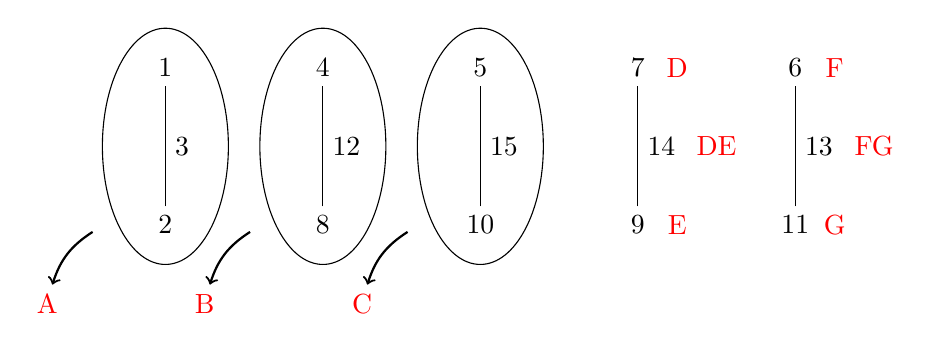
\begin{tikzpicture}
	% Define 1 2 3
	\node (Node2) at (0,0) {2};
	\node (Middle12) at (0,1) {};
	\node (Eclipse12) at (-0.8,0) {};
	\node (Node1) at (0,2) {1};
	\node[red] (A) at (-1.5, -1) {A};

	\draw (Node2) -- node[midway, right] {3} (Node1);
	\draw (Middle12) ellipse (0.8cm and 1.5cm);
	\draw[->, thick] (Eclipse12) to[bend right=20] (A);
	
	
	% Define 4 8 12
	\node (Node8) at (2,0) {8};
	\node (Middle84) at (2,1) {};
	\node (Eclipse84) at (1.2,0) {};
	\node (Node4) at (2,2) {4};
	\node[red] (B) at (0.5, -1) {B};
	
	\draw (Node8) -- node[midway, right] {12} (Node4);
	\draw (Middle84) ellipse (0.8cm and 1.5cm);
	\draw[->, thick] (Eclipse84) to[bend right=20] (B);
	
	% Define 5 15 10
	\node (Node10) at (4,0) {10};
	\node (Middle105) at (4,1) {};
	\node (Eclipse105) at (3.2,0) {};
	\node (Node5) at (4,2) {5};
	\node[red] (C) at (2.5, -1) {C};
	
	\draw (Node10) -- node[midway, right] {15} (Node5);
	\draw (Middle105) ellipse (0.8cm and 1.5cm);
	\draw[->, thick] (Eclipse105) to[bend right=20] (C);
	
	% Define 7 9 14
	\node (Node9) at (6,0) {9};
	\node (Node7) at (6,2) {7};
	\node[red] (E) at (6.5,0) {E};
	\node[red] (D) at (6.5,2) {D};
	\node[red] (DE) at (7,1) {DE};
	
	\draw (Node9) -- node[midway, right] {14} (Node7);
	
	
	% Define 6 11 13
	\node (Node11) at (8,0) {11};
	\node (Node6) at (8,2) {6};
	\node[red] (G) at (8.5,0) {G};
	\node[red] (F) at (8.5,2) {F};
	\node[red] (FG) at (9,1) {FG};
	
	\draw (Node11) -- node[midway, right] {13} (Node6);
\end{tikzpicture}
\caption{Modified Linear Graph to fit our needs}
\end{figure}


Combining columns 1 2 3 to A, 4 8 12 to B and 5 10 15 to C can be done using these rules:

\begin{figure}[H]
	\centering
	\begin{tabular}{ |ccccccc|  }
		\hline
		\multicolumn{3}{|c}{ OLD COLUMN } & & & & NEW COLUMN \\
		\hline
		& 1 & 1 & & -> & & 1\\
		& 1 & 2 & & -> & & 2\\
		& 2 & 1 & & -> & & 3\\
		& 2 & 2 & & -> & & 4\\
		\hline
	\end{tabular}
	\caption{Rules taken from \cite{roy_primer_1990}}
\end{figure}

\begin{figure}[H]
	\centering
	\begin{tabular}{ |c||cccc|cccc|cccc|  }
		\hline
		NO.& 1 & 2 & & \sout{3} & 4 & 8 & &  \sout{12} & 5 & 10 & &  \sout{15}\\
		\hline
		1  & \multicolumn{4}{c}{\sout{1 1} > 1 } & \multicolumn{4}{|c|}{\sout{1 1} > 1 } & \multicolumn{4}{c|}{\sout{1 1} > 1 }\\
		2  & \multicolumn{4}{c}{\sout{1 1} > 1 } & \multicolumn{4}{|c|}{\sout{1 2} > 2 } & \multicolumn{4}{c|}{\sout{1 2} > 2 }\\
		3  & \multicolumn{4}{c}{\sout{1 1} > 1 } & \multicolumn{4}{|c|}{\sout{2 1} > 3 } & \multicolumn{4}{c|}{\sout{2 1} > 3 }\\
		4  & \multicolumn{4}{c}{\sout{1 1} > 1 } & \multicolumn{4}{|c|}{\sout{2 2} > 4 } & \multicolumn{4}{c|}{\sout{2 2} > 4 }\\
		5  & \multicolumn{4}{c}{\sout{1 2} > 2 } & \multicolumn{4}{|c|}{\sout{1 1} > 1 } & \multicolumn{4}{c|}{\sout{1 2} > 2 }\\
		6  & \multicolumn{4}{c}{\sout{1 2} > 2 } & \multicolumn{4}{|c|}{\sout{1 2} > 2 } & \multicolumn{4}{c|}{\sout{1 1} > 1 }\\
		7  & \multicolumn{4}{c}{\sout{1 2} > 2 } & \multicolumn{4}{|c|}{\sout{2 1} > 3 } & \multicolumn{4}{c|}{\sout{2 2} > 4 }\\
		8  & \multicolumn{4}{c}{\sout{1 2} > 2 } & \multicolumn{4}{|c|}{\sout{2 2} > 4 } & \multicolumn{4}{c|}{\sout{2 1} > 3 }\\
		9  & \multicolumn{4}{c}{\sout{2 1} > 3 } & \multicolumn{4}{|c|}{\sout{1 1} > 1 } & \multicolumn{4}{c|}{\sout{2 1} > 3 }\\
		10 & \multicolumn{4}{c}{\sout{2 1} > 3 } & \multicolumn{4}{|c|}{\sout{1 2} > 2 } & \multicolumn{4}{c|}{\sout{2 2} > 4 }\\
		11 & \multicolumn{4}{c}{\sout{2 1} > 3 } & \multicolumn{4}{|c|}{\sout{2 1} > 3 } & \multicolumn{4}{c|}{\sout{1 1} > 1 }\\
		12 & \multicolumn{4}{c}{\sout{2 2} > 3 } & \multicolumn{4}{|c|}{\sout{2 2} > 4 } & \multicolumn{4}{c|}{\sout{1 2} > 2 }\\
		13 & \multicolumn{4}{c}{\sout{2 2} > 4 } & \multicolumn{4}{|c|}{\sout{1 1} > 1 } & \multicolumn{4}{c|}{\sout{2 2} > 4 }\\
		14 & \multicolumn{4}{c}{\sout{2 2} > 4 } & \multicolumn{4}{|c|}{\sout{1 2} > 2 } & \multicolumn{4}{c|}{\sout{2 1} > 3 }\\
		15 & \multicolumn{4}{c}{\sout{2 2} > 4 } & \multicolumn{4}{|c|}{\sout{2 1} > 3 } & \multicolumn{4}{c|}{\sout{1 2} > 2 }\\
		16 & \multicolumn{4}{c}{\sout{2 2} > 4 } & \multicolumn{4}{|c|}{\sout{2 2} > 4 } & \multicolumn{4}{c|}{\sout{1 1} > 1 }\\
		\hline
	\end{tabular}
	\caption{Building 4 Level columns from 2 Level columns}
\end{figure}

After removing the old and inserting the new columns in the table and transcoding 7 to D, 9 to E, 14 to DE, 6 to F, 11 to G and 13 to FG, we have the following table:

\begin{figure}[H]
	\centering
	\begin{tabular}{ |c||c|c|c|c|c|c|c|c|c|  }
		\hline
		NO.& A & B & C & D & E & F & G & FG& DE\\
		\hline
		1  & 1 & 1 & 1 & 1 & 1 & 1 & 1 & 1 & 1\\
		2  & 1 & 2 & 2 & 1 & 2 & 1 & 2 & 2 & 2\\
		3  & 1 & 3 & 3 & 2 & 1 & 2 & 1 & 2 & 2\\
		4  & 1 & 4 & 4 & 2 & 2 & 2 & 2 & 1 & 1\\
		5  & 2 & 1 & 2 & 2 & 1 & 2 & 2 & 1 & 2\\
		6  & 2 & 2 & 1 & 2 & 2 & 2 & 1 & 2 & 1\\
		7  & 2 & 3 & 4 & 1 & 1 & 1 & 2 & 2 & 1\\
		8  & 2 & 4 & 3 & 1 & 2 & 1 & 1 & 1 & 2\\
		9  & 3 & 1 & 3 & 2 & 2 & 1 & 2 & 2 & 1\\
		10 & 3 & 2 & 4 & 2 & 1 & 1 & 1 & 1 & 2\\
		11 & 3 & 3 & 1 & 1 & 2 & 2 & 2 & 1 & 2\\
		12 & 3 & 4 & 2 & 1 & 1 & 2 & 1 & 2 & 1\\
		13 & 4 & 1 & 4 & 1 & 2 & 2 & 1 & 2 & 2\\
		14 & 4 & 2 & 3 & 1 & 1 & 2 & 2 & 1 & 1\\
		15 & 4 & 3 & 2 & 2 & 2 & 1 & 1 & 1 & 1\\
		16 & 4 & 4 & 1 & 2 & 1 & 1 & 2 & 2 & 2\\
		\hline
	\end{tabular}
	\caption{Final version of used Taguchi orthogonal array}
\end{figure}


\subsection{Analysing the results}

This now can be used for running all the needed testcases (the interaction columns can be ignored until the evaluation). Simply exchange all levels in the table with the corresponding setting from table \ref{table:hyperparameter_tuning:settings_to_level}. We will repeat every setting 8 times. These are the results:


\begin{figure}[H]
	\centering
	\begin{tabular}{ |c||c|c|c|c|c|c|c|c|  }
		\hline
		NO.& rep1 & rep2 & rep3 & rep4 & rep5 & rep6 & rep7 & rep8\\
		\hline
		1  & 1000 & 1000 & 1000 & 1000 & 1000 & 1000 & 1000 & 1000\\
		2  & 1000 & 1000 & 1000 & 1000 & 1000 & 1000 & 1000 & 1000\\
		3  & 1000 & 1000 & 1000 & 1000 & 1000 & 1000 & 1000 & 1000\\
		4  & 1000 & 1000 & 1000 & 1000 & 1000 & 1000 & 1000 & 1000\\
		5  & 1000 & 1000 & 1000 & 1000 & 1000 & 1000 & 1000 & 1000\\
		6  & 1000 & 1000 & 1000 & 1000 & 1000 & 1000 & 1000 & 1000\\
		7  & 1000 & 1000 & 1000 & 1000 & 1000 & 1000 & 1000 & 1000\\
		8  & 1000 & 1000 & 1000 & 1000 & 1000 & 1000 & 1000 & 1000\\
		9  & 1000 & 1000 & 1000 & 1000 & 1000 & 1000 & 1000 & 1000\\
		10 & 1000 & 1000 & 1000 & 1000 & 1000 & 1000 & 1000 & 1000\\
		11 & 1000 & 1000 & 1000 & 1000 & 1000 & 1000 & 1000 & 1000\\
		12 & 1000 & 1000 & 1000 & 1000 & 1000 & 1000 & 1000 & 1000\\
		13 & 1000 & 1000 & 1000 & 1000 & 1000 & 1000 & 1000 & 1000\\
		14 & 1000 & 1000 & 1000 & 1000 & 1000 & 1000 & 1000 & 1000\\
		15 & 1000 & 1000 & 1000 & 1000 & 1000 & 1000 & 1000 & 1000\\
		16 & 1000 & 1000 & 1000 & 1000 & 1000 & 1000 & 1000 & 1000\\
		\hline
	\end{tabular}
	\caption{List of results}
\end{figure}



\subsubsection{ANOVA}

Due to our number of repetitions, the number of DOF increases according to the following equation (taken from \cite{roy_primer_1990}):

\begin{equation} \label{full DOF}
	\begin{split}
		DOF & = totalNumberOfResults - 1 \\
		& = numberOfTrials * numberOfRepetitions - 1 \\
		& = 16 * 8 - 1 = 127
	\end{split}
\end{equation}



Calculating ANOVA can be done using R: \todo{Cite book from Gabriel}
\begin{lstlisting}[language=R]
	# pivot the results, so that the table has 8 times the rows
	taguchi.combined_pivoted <- taguchi.combined %>% pivot_longer(cols = starts_with("min_"), values_to = "results")

	# run anova analysis
	anova <- aov(results ~ factor(A) + factor(B) + factor(C) + factor(D) * factor(E) + factor(F) * factor(G), data = taguchi.combined_pivoted)
	summary(anova)
\end{lstlisting}

After pooling, we can run anova again:
\begin{lstlisting}[language=R]
	anova <- aov(results ~ factor(A) + factor(B) + factor(C) + factor(D) * factor(E) + factor(F) * factor(G), data = taguchi.combined_pivoted)
	summary(anova)
\end{lstlisting}

This will result in the following table:

\begin{figure}[H]
	\centering
	\begin{tabular}{ |cccccc|  }
		\hline
		Column 		& DF & Sum Sq & Mean Sq & F value & p value\\
		\hline
		1  & A 		& 3 & 1000 & 1000 & 1000\\
		2  & B 		& 3 & 1000 & 1000 & 1000\\
		3  & C 		& 3 & 1000 & 1000 & 1000\\
		4  & D 		& 1 & 1000 & 1000 & 1000\\
		5  & E 		& 1 & 1000 & 1000 & 1000\\
		6  & F 		& 1 & 1000 & 1000 & 1000\\
		7  & G 		& 1 & 1000 & 1000 & 1000\\
		8  & DxE 	& 1 & 1000 & 1000 & 1000\\
		9  & FxG 	& 1 & 1000 & 1000 & 1000\\
		\hline
		\multicolumn{2}{|c}{Residuals} &  & 1000 & 1000 & 1000\\
		\hline
	\end{tabular}
	\caption{ANOVA results}
\end{figure}

\subsubsection{Main-effects and interaction chart}\todo{Main-effects or main-effect}

According to \cite{yang_design_2009}, "The main-effects chart is a plot of average responses at different levels of a factor versus the factor levels" and the calculation" of main-effect charts and iteration charts are the same as those of classical experimental data analysis".

For every factor, sum up the mean of the results per level, then divide by the number of runs per level. This is the calculation for D:
\todo{Insert calculation for d}

The resulting main-effect charts can be seen here:
\begin{figure}[H] 
	\begin{minipage}[b]{0.33\linewidth}
		\centering
		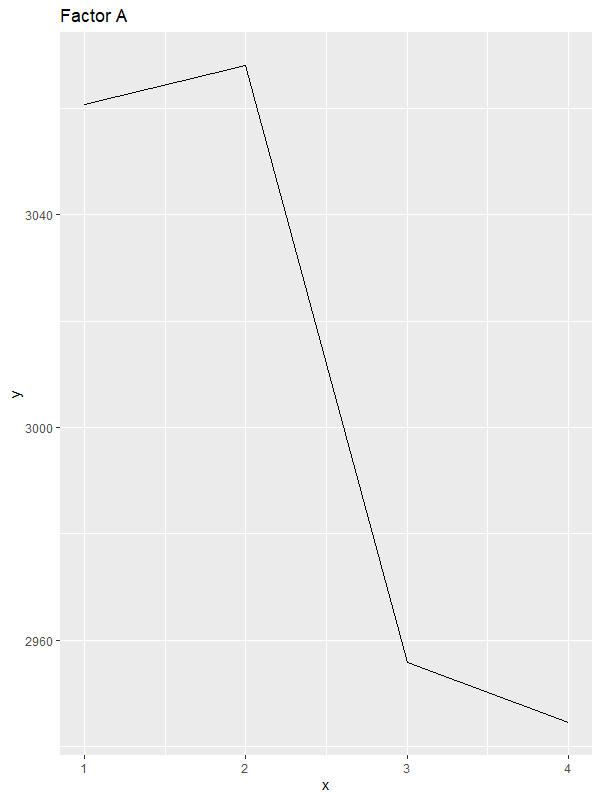
\includegraphics[width=1\linewidth]{simulations/taguchi/plots/main_effect_a} 
	\end{minipage}%%
	\begin{minipage}[b]{0.33\linewidth}
		\centering
		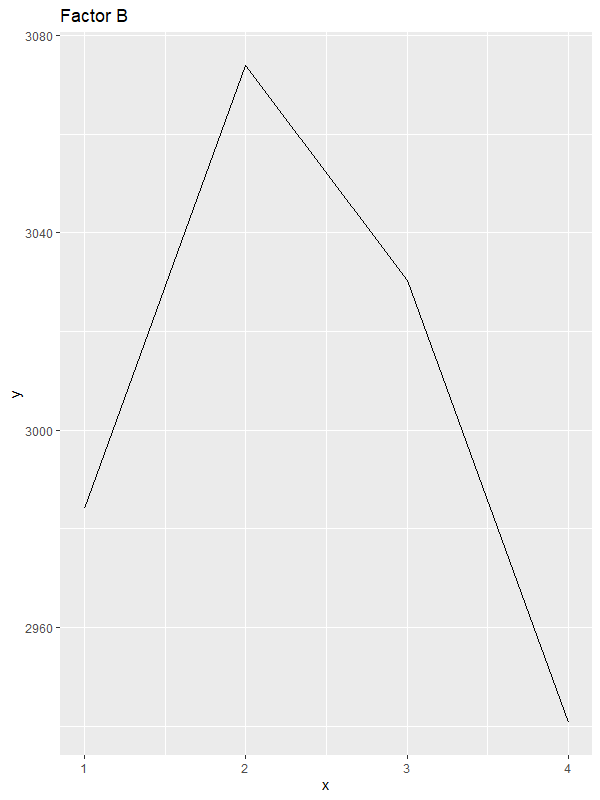
\includegraphics[width=1\linewidth]{simulations/taguchi/plots/main_effect_b} 
	\end{minipage}%%
	\begin{minipage}[b]{0.33\linewidth}
		\centering
		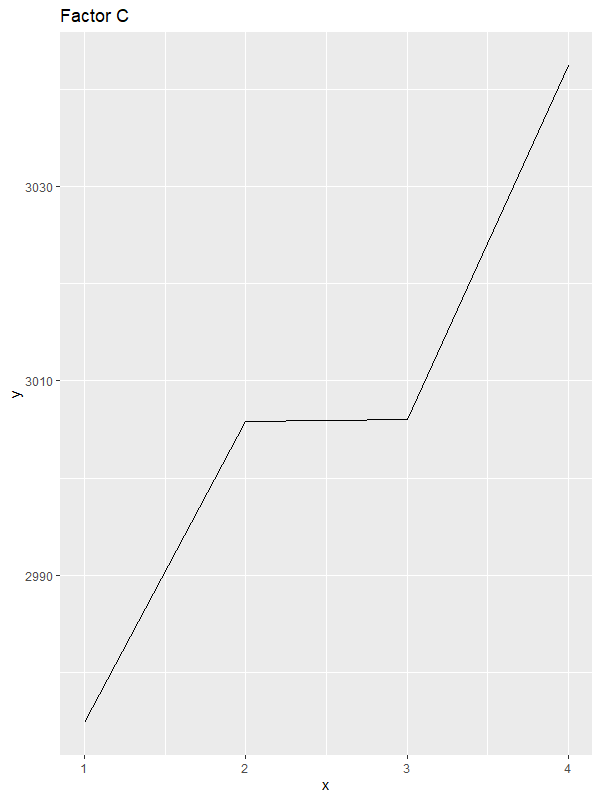
\includegraphics[width=1\linewidth]{simulations/taguchi/plots/main_effect_c} 
	\end{minipage}
	
	\begin{minipage}[b]{0.33\linewidth}
		\centering
		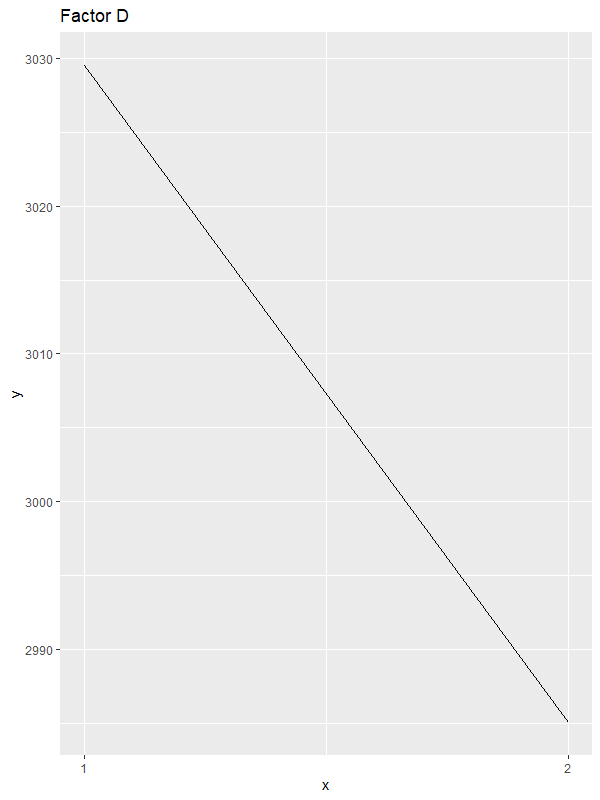
\includegraphics[width=1\linewidth]{simulations/taguchi/plots/main_effect_d} 
	\end{minipage}%% 
	\begin{minipage}[b]{0.33\linewidth}
		\centering
		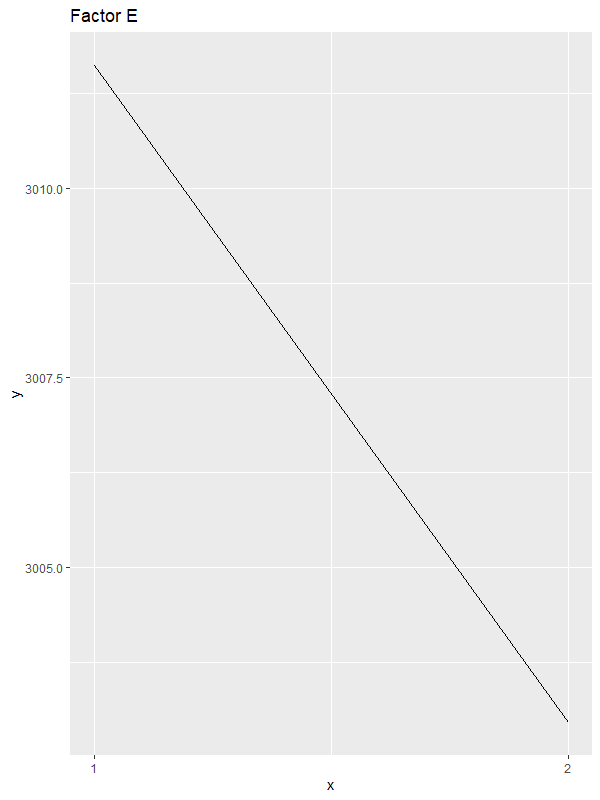
\includegraphics[width=1\linewidth]{simulations/taguchi/plots/main_effect_e} 
	\end{minipage}%% 
	\begin{minipage}[b]{0.33\linewidth}
		\centering
		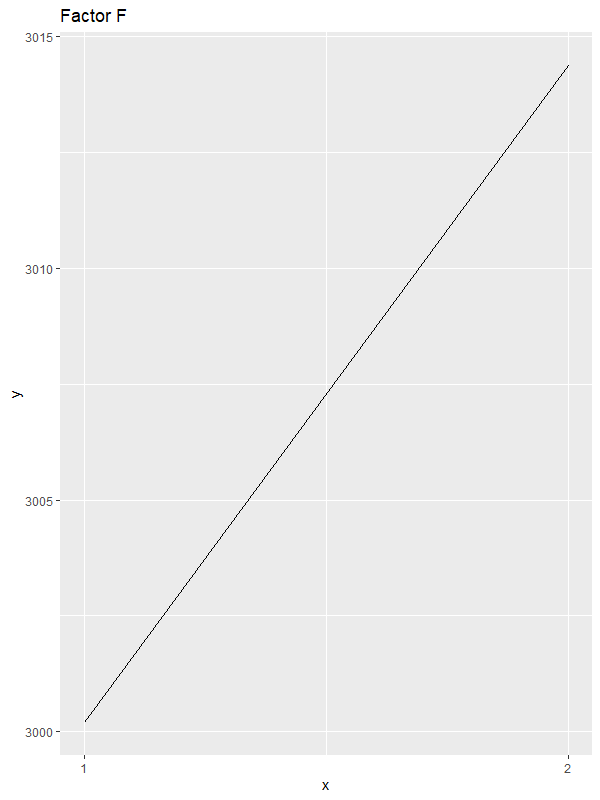
\includegraphics[width=1\linewidth]{simulations/taguchi/plots/main_effect_f} 
	\end{minipage}
	
	\begin{minipage}[b]{0.33\linewidth}
		\centering
		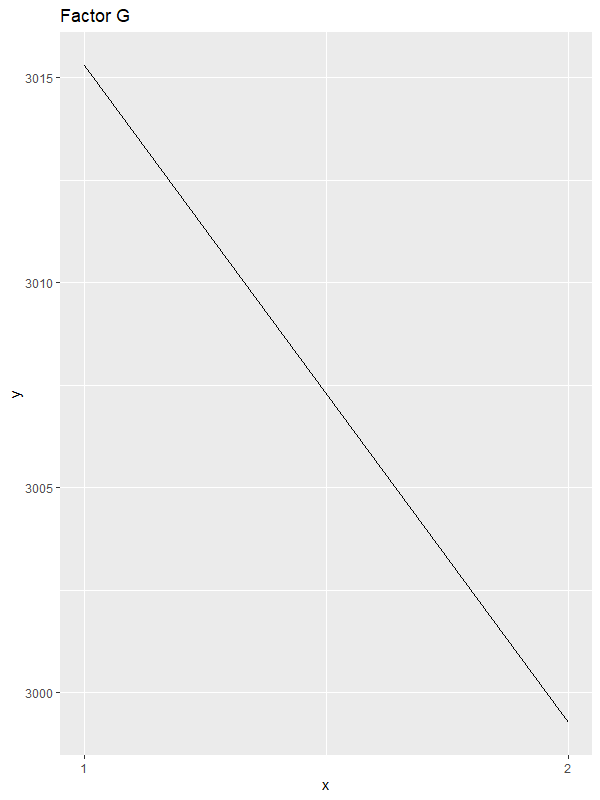
\includegraphics[width=1\linewidth]{simulations/taguchi/plots/main_effect_g} 
	\end{minipage}
	\caption{Main-effect charts}
\end{figure}



Similaly, the interactions are calculated like this:
\todo{Insert example calculation of interaction}


The resulting interaction charts can be seen here:
\begin{figure}[H] 
	\begin{minipage}[b]{0.33\linewidth}
		\centering
		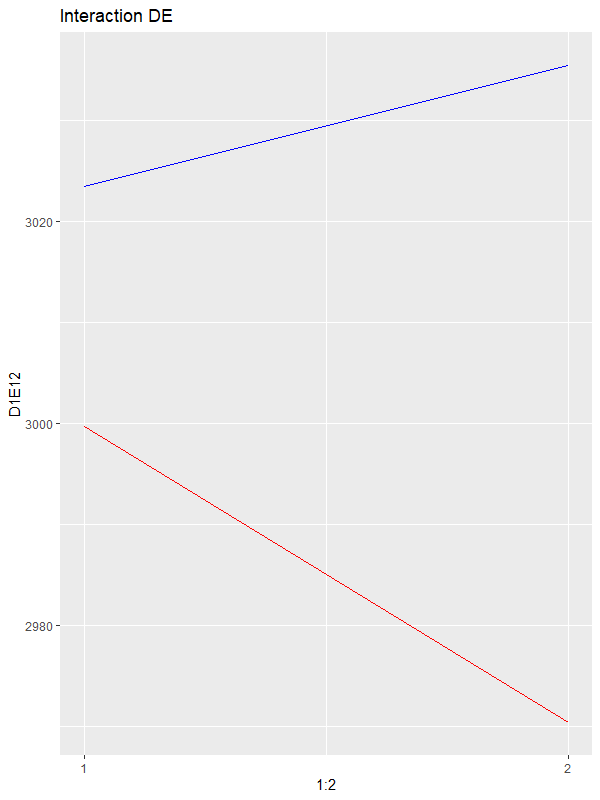
\includegraphics[width=1\linewidth]{simulations/taguchi/plots/interaction_de} 
	\end{minipage}%%
	\begin{minipage}[b]{0.33\linewidth}
		\centering
		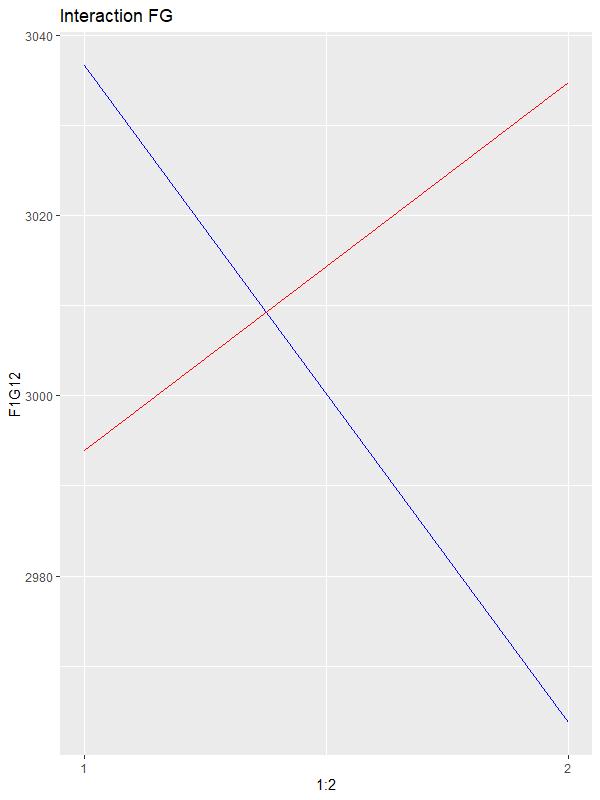
\includegraphics[width=1\linewidth]{simulations/taguchi/plots/interaction_fg} 
	\end{minipage}
	\caption{Interaction charts}
\end{figure}



\paragraph{Best factor level selection and optimal performance level prediction (Take from yang\_design\_2009, so reformulate)}
